%FILE: coordinates.tex

\chapter{Ice Element Location and Position}

\section{Introduction}

Let an ice element be considered as a flat (2D) rigid body in a form
of convex polygon moving on a spherical surface. The goals of this
chapter are
\begin{itemize}
  \item Find a suitable description of position and orientation of the
    ice element;
  \item Derive position integraion equations;
  \item Build an integration numerical algorithm to update position
    and orientation of the ice element;
  \item Describe coordinate transformations used in the model.
\end{itemize}

\section{Equivalence to 3D Rigid Body Rotations}

\begin{figure}
  \center
  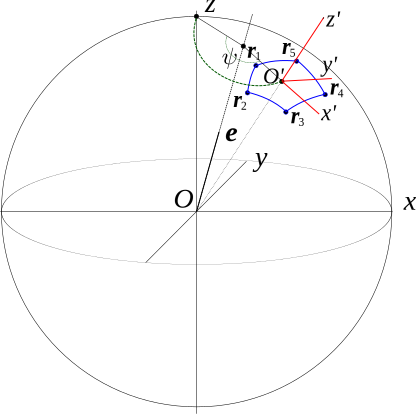
\includegraphics[width=0.5\textwidth]{pics/sphere-dynamics.pdf}
  \caption{Coordinates}
  \label{fig:coordinates}
\end{figure}

It is easy to see (but not so easy to find out) that the motion of an
ice element on the surface of a sphere is equivalent to a rotation of
a rigid body around the center of the sphere. Such a rigid body can be
considered to be a pendulum with a massive weight to be a material
polygon which center of mass is connected to the center of the sphere
by a massless rod. The center of the sphere does not move and is a
center of the rotation. This set up is shown in
Figure.~\ref{fig:coordinates}.

It also can be visualized as a rotation of the rigid sphere shell
around its center with all the mass concentrated inside a single
polygon patch -- an ice element.

The representation of an ice element as a 3D constrained rotating
rigid body provides a useful instrument to describe exact position and
orientation of an ice element. The rigid body rotation around a point
can be described by unit quaternions a.k.a
versors~\cite{bib:graf2008quaternions, bib:waldvogel2008quaternions,
  bib:arribas2006quaternions, bib:nemes2013perturbed}. The main
advantage of using quaternions instead of, say, spherical coordinates
with a rotation angle is that every point on a sphere is treated
exactly the same way as any other point. The density of coordinate
lines do not change from point to point and no critical points are
present. The quaternion representation also allows to perfom many
coordinate transformations without involving trigonometry, store
orientation information very compactly, and the formulas of all
necessary operations are simple and short. \textbf{A single quaternion
  is sufficient to uniqly describe the position and orientation of an
  ice element}.

%----------------------------------------------------------------------
\section{Coordinate Systems and Frames}\label{sec:frames}

When describing different values such as positions or vectors we use 2
different types of reference points or ``frames'' depending on
convenience:
\begin{itemize}
\item Global Frame, connected to the Earth and rotating with the
  Earth;
\item Local Frames, a reference point connected to a particular ice
  element.
\end{itemize}

For describing elements in Global Frame, we use 3 different coordinate
system:
\begin{itemize}
\item Geographical coordinates (latitude $\varphi$ and longitude
  $\lambda$). They used only for import or export elements and never
  used internally. We provide trasformation from and to geographical
  coordinates.
\item Spherical coordinates ($\phi=\lambda$, $\theta=\pi/2-\varphi$).
\item 3D extrinsic Cartesian coordinates $(x',y',z')$.  Its center
  coincides with the center of the Earth $O$, $z'$ is directed along
  Earth's axis of rotation towards the North, $x'$ direction is a
  direction to 0 meridian, and $y'$ direction is chosen perpendicular
  to $x'$ and $z'$ to form a right coordinate system. These
  coordinates satisfy the constrain ${x'}^2+{y'}^2+{z'}^2=R^2$.
\item 3D normalized (dimensionless) extrinsic Cartesian coordinates
  $(x,y,z)$. Same as above but all projected to a unit sphere such
  that ${x}^2+{y}^2+{z}^2=1$.  \textit{These are the main global coordinates
  internally used in the Core for all the computations.}
\end{itemize}

We use Global Frame only when considering interaction between two ice
elements. In all other cases we transform global coordinates into a
local frame first and then produce the computations.

The transformation between extrinsic coordinates and
geographic/spherical coordinates are performed using the following
formulas:
\begin{equation}\label{eq:extrinsic}
  \left\{
  \begin{aligned}
    \theta &= \pi/2 - \varphi,\\
    \phi &=\lambda.\\
  \end{aligned}
  \right.\qquad\left\{
  \begin{aligned}
    x &= \sin\theta\cos\phi, \\
    y &= \sin\theta\sin\phi, \\
    z &= \cos\theta.\\
  \end{aligned}
  \right.
\end{equation}

Local coordinates $(X,Y,Z)$ are the coordinates that have its center
in the center of mass of the ice element. The axis are directed such
that they would coincide with global frame normalized extrinsic
coordinates $(x,y,z)$ after application of the rotation described by
the quaternion $\untqtrn{q}$ linked to the ice element.

Global extrinsic coordinates for any point $\pnt{p}$ are restored from
local coordinates $\pnt{P}$ by applying the rotation matrix recovered
from quaternion:
\begin{equation}
  \pnt{p} = \mtr{R}(\untqtrn{q})\cdot\pnt{P}
\end{equation}
Rotation matrix can be recovered from quaternion as described in
Section~\ref{sec:rotquat}.

%----------------------------------------------------------------------
\section{Initial Frame Relation}

To relate two different frames, we have to introduce initial
quaternion $\untqtrn{q}_0$. Later we will provide a first order
differential equation for the evolution of the quaternion. However, we
have to find this initial quaternion to be able to resolve the
evolution.

We found a simple way to set this initial position
quaternion. Initially, we have initial coordinates of the polygon
representing the ice elements in some of Global Frame coordinates. To
find initial quaternion we will do the following
\begin{enumerate}
\item Find center of mass of the polygon in global frame.
\item Find a quaternion such that when applied, it moves the center of
  mass into the North Pole. There are an infinite number of such
  rotation quaternions, so we pick one.
\item We introduce initial local coordinates based on this initial
  quaternion such that they will coincide with extrinsic coordinates
  after the transformation. All vertices coordinates $\pnt{P}_i =
  (X_i,Y_i,Z_i)$ are computed then. They will never change with time.
\end{enumerate}

There is an uncertainty in quaternion choice that initially would
transpose the center of ice element into North pole. Let us choose the
quaternion that transpose the center of the ice element as follows.

Suppose we have coordinates of the center of mass in Global Frame in
Extrinsic coordinates: $\pnt{c}=(c_x,c_y,c_z)$, then we restore the
transformation as a rotation along big circle to match $\pnt{c}$ with
North Pole as follows:
\begin{equation}
  \untqtrn{q_0} = \cos{\theta/2} + \untvct{e}\sin{\theta/2},\qquad \untvct{e} =
  \vct{c}\times\untvct{e_z}/|\vct{c}\times\untvct{e_z}|, \quad \theta =
  \arccos{c_z/|\vct{c}|}.
\end{equation}
$\theta$ is spherical coordinates of $\pnt{c}$. The rotation axis is
perpendicular to $\pnt{c}$ and direction to the North. Reminder: we
use a convention that vectors and scalars are all a subset of
quaternions and can be added to each other to make a new quaternion.

%% -------------------------------------------------------------------

\section{Position Update Equation}

Suppose we know the vector of angular velocity of our ``pendulum''
$\vec{\omega}$. Please, notice that this is 3D angular velocity
vector, not a rotation rate of the ice element. Later we will see how
to calculate it from the velocity and rotation rate of the ice element
itself. In this case we have the following expression for updating
orientation quaternion
\begin{equation}
  \dot{\untqtrn{q}} = \frac{1}{2}\vct{\omega}\circ\untqtrn{q}.
\end{equation}
Where $\dot q=dq/dt$.  Let $\vct{\Omega}$ be the same angular velocity
vector expressed in Local frame
coordinates. Using~\eqref{eq:transform} we can derive the main
position equation:
\begin{equation}\label{eq:positionomega}
  \dot{\untqtrn{q}} = \frac{1}{2}\untqtrn{q}\circ\vct{\Omega},
\end{equation}
While developing \coupi\/ we created a very neat scheme to solve this
type of equations. This scheme will be described here later based on
\coupi\/ documentation.

%% -------------------------------------------------------------------

\section{Placement Numerical Integration}

Let us describe the numerical solution of the
equation~\eqref{eq:positionomega}.  

Let $\vct{\Omega}^{n+1/2} = \vct{\Omega}(t+\Delta t/2)$ (and this
value we will actually find on the dynamic stage),
$\untqtrn{q}^{n}=\untqtrn{q}(t)$,
$\untqtrn{q}^{n+1}=\untqtrn{q}(t+\Delta t)$. The 2nd order scheme for
the equation above will be
\begin{equation}
  \untqtrn{q}^{n+1} = \untqtrn{q}^n + \frac{\Delta t}{4} 
  (\untqtrn{q}^{n}+\untqtrn{q}^{n+1})\circ
  \vct{\Omega}^{n+1/2}.
\end{equation}
Collecting all next step values on the left side and taking into
account that quaternion product is not commutative, we have
\begin{equation}\label{eq:scheme}
  \untqtrn{q}^{n+1}\circ\left( 1 - \frac{\Delta t}{4}\vct{\Omega}\right) = 
  \untqtrn{q}^{n}\circ\left( 1 + \frac{\Delta t}{4}\vct{\Omega}\right).
\end{equation}
We removed index $n+1/2$ from $\vct{\Omega}$ to make it easier to
read. Brackets in~\eqref{eq:scheme} are conjugate
quaternions. Using relation $\untqtrn{q}\circ\untqtrn{\bar{q}} = |q|^2$ we have
\begin{equation}
  \untqtrn{q}^{n+1}\circ\left( 1 - \frac{\Delta
    t}{4}\vct{\Omega}\right)\circ\left( 1 + \frac{\Delta
    t}{4}\vct{\Omega}\right) = \untqtrn{q}^{n}\circ\left( 1 + \frac{\Delta
    t}{4}\vct{\Omega}\right)^2.
\end{equation}
\begin{equation}
  \untqtrn{q}^{n+1}\left( 1 +\frac{ \Omega^2\,\Delta
    t^2}{16}\right) = \untqtrn{q}^{n}\circ\left( 1 + \frac{\Delta
    t}{4}\vct{\Omega}\right)^2.
\end{equation}
\begin{equation}
  \untqtrn{q}^{n+1} = \untqtrn{q}^{n}\circ\left( 1 + \frac{\Delta
    t}{4}\vct{\Omega}\right)^2 / \left( 1 +\frac{ \Omega^2\,\Delta
    t^2}{16}\right)
\end{equation}
For any vector $\vct{a}$ using product Eq.~\eqref{eq:quatproduct} we
have
\begin{equation}
  (1+\vct{a})^2 = (1+\vct{a})\circ(1+\vct{a}) =
  1 - a^2 + 2\vct{a}.
\end{equation}
Then, we have
\begin{equation}
  \untqtrn{q}^{n+1} = \untqtrn{q}^{n} \circ \left(1 - \frac{\Omega^2\,\Delta t^2}{16} +
  \frac{\Delta t}{2}\,\vct{\Omega} \right) / \left( 1 +\frac{ \Omega^2\,\Delta
    t^2}{16}\right)
\end{equation}
Let us introduce the following quaternion
\begin{equation}
  \untqtrn{p} = \left(1 - \frac{\Omega^2\,\Delta t^2}{16} + \frac{\Delta
    t}{2}\,\vct{\Omega} \right) / \left( 1 +\frac{ \Omega^2\,\Delta
    t^2}{16}\right),
\end{equation}
then integration formula will have the form
\begin{equation}
  \untqtrn{q}^{n+1} = \untqtrn{q}^{n} \circ \untqtrn{p}.
\end{equation}
Computation wise it is a significant improvement over
\cite{bib:Walton-Braun-1993} quaternion integration formula or
trigonometric approach like in \cite{bib:gpugems3-harada-2008}.

It is easy to see that $|\untqtrn{p}|=1$ and hence this formula does not
change the absolute value of unit quaternion. However, round-off
errors might accumulate in time shifting the absolute value of
$\untqtrn{q}$ from 1. To ensure we are working within unit quaternion
algebra, a renormalization should be done occasionally
\begin{equation}
  \untqtrn{q} \leftarrow \untqtrn{q}/|q|.
\end{equation}

